\documentclass[tikz,border=5mm]{standalone}
\usetikzlibrary{shapes.arrows, positioning}

\begin{document}
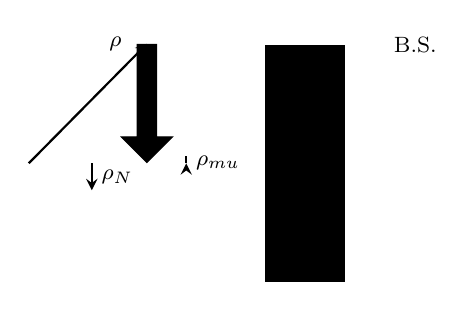
\begin{tikzpicture}[
    >=stealth,
    node distance=1.5cm,
    arrow/.style={single arrow, draw, fill=black, minimum height=1cm, single arrow head extend=.2cm},
    bs/.style={rectangle, draw, fill=black, minimum width=1cm, minimum height=3cm},
    dotline/.style={dotted, gray, thick},
]

% Draw amplifier
\node (amp) [arrow, rotate=-90, minimum height=1.5cm, anchor=east] at (0,0) {};
\node[right=of amp.east, font=\footnotesize] {Amp};

% Draw beam splitter
\node (bs) [bs, right=of amp.east] {};
\node[right=0.5cm of bs.north east, font=\footnotesize] {B.S.};

% Input arrow
\draw[->, thick] (-1.5,0) -- (amp.west);
\node[left=0.2cm of amp.west, font=\footnotesize] {$\rho$};

% Output arrows
\foreach \i/\y in {1/1.2, mu/0, N/-1.2}{
    \draw[->, thick] ([xshift=0.5cm]\y cm,0) -- ([xshift=0.5cm]\y cm,0 |- bs.\y cm);
    \node[dotline, xshift=0.5cm, yshift=0.1cm] (\i-vert) at (\y cm, 0) {};
    \node[dotline, xshift=0.5cm, yshift=-0.1cm] (\i-horz) at (\y cm, 0 |- bs.\y cm) {};
    \path (\i-vert.south) -- (\i-horz.north) node[midway, right, font=\footnotesize] {$\rho_{\i}$};
}

\end{tikzpicture}
\end{document}